\documentclass[]{ctexbook}
\usepackage{lmodern}
\usepackage{amssymb,amsmath}
\usepackage{ifxetex,ifluatex}
\usepackage{fixltx2e} % provides \textsubscript
\ifnum 0\ifxetex 1\fi\ifluatex 1\fi=0 % if pdftex
  \usepackage[T1]{fontenc}
  \usepackage[utf8]{inputenc}
\else % if luatex or xelatex
  \ifxetex
    \usepackage{xltxtra,xunicode}
  \else
    \usepackage{fontspec}
  \fi
  \defaultfontfeatures{Ligatures=TeX,Scale=MatchLowercase}
\fi
% use upquote if available, for straight quotes in verbatim environments
\IfFileExists{upquote.sty}{\usepackage{upquote}}{}
% use microtype if available
\IfFileExists{microtype.sty}{%
\usepackage{microtype}
\UseMicrotypeSet[protrusion]{basicmath} % disable protrusion for tt fonts
}{}
\usepackage[b5paper,tmargin=2.5cm,bmargin=2.5cm,lmargin=3.5cm,rmargin=2.5cm]{geometry}
\usepackage[unicode=true]{hyperref}
\PassOptionsToPackage{usenames,dvipsnames}{color} % color is loaded by hyperref
\hypersetup{
            pdftitle={Overleaf功能介绍},
            pdfauthor={wang},
            colorlinks=true,
            linkcolor=Maroon,
            citecolor=Blue,
            urlcolor=Blue,
            breaklinks=true}
\urlstyle{same}  % don't use monospace font for urls
\usepackage{natbib}
\bibliographystyle{apalike}
\usepackage{color}
\usepackage{fancyvrb}
\newcommand{\VerbBar}{|}
\newcommand{\VERB}{\Verb[commandchars=\\\{\}]}
\DefineVerbatimEnvironment{Highlighting}{Verbatim}{commandchars=\\\{\}}
% Add ',fontsize=\small' for more characters per line
\usepackage{framed}
\definecolor{shadecolor}{RGB}{248,248,248}
\newenvironment{Shaded}{\begin{snugshade}}{\end{snugshade}}
\newcommand{\AlertTok}[1]{\textcolor[rgb]{0.94,0.16,0.16}{#1}}
\newcommand{\AnnotationTok}[1]{\textcolor[rgb]{0.56,0.35,0.01}{\textbf{\textit{#1}}}}
\newcommand{\AttributeTok}[1]{\textcolor[rgb]{0.77,0.63,0.00}{#1}}
\newcommand{\BaseNTok}[1]{\textcolor[rgb]{0.00,0.00,0.81}{#1}}
\newcommand{\BuiltInTok}[1]{#1}
\newcommand{\CharTok}[1]{\textcolor[rgb]{0.31,0.60,0.02}{#1}}
\newcommand{\CommentTok}[1]{\textcolor[rgb]{0.56,0.35,0.01}{\textit{#1}}}
\newcommand{\CommentVarTok}[1]{\textcolor[rgb]{0.56,0.35,0.01}{\textbf{\textit{#1}}}}
\newcommand{\ConstantTok}[1]{\textcolor[rgb]{0.00,0.00,0.00}{#1}}
\newcommand{\ControlFlowTok}[1]{\textcolor[rgb]{0.13,0.29,0.53}{\textbf{#1}}}
\newcommand{\DataTypeTok}[1]{\textcolor[rgb]{0.13,0.29,0.53}{#1}}
\newcommand{\DecValTok}[1]{\textcolor[rgb]{0.00,0.00,0.81}{#1}}
\newcommand{\DocumentationTok}[1]{\textcolor[rgb]{0.56,0.35,0.01}{\textbf{\textit{#1}}}}
\newcommand{\ErrorTok}[1]{\textcolor[rgb]{0.64,0.00,0.00}{\textbf{#1}}}
\newcommand{\ExtensionTok}[1]{#1}
\newcommand{\FloatTok}[1]{\textcolor[rgb]{0.00,0.00,0.81}{#1}}
\newcommand{\FunctionTok}[1]{\textcolor[rgb]{0.00,0.00,0.00}{#1}}
\newcommand{\ImportTok}[1]{#1}
\newcommand{\InformationTok}[1]{\textcolor[rgb]{0.56,0.35,0.01}{\textbf{\textit{#1}}}}
\newcommand{\KeywordTok}[1]{\textcolor[rgb]{0.13,0.29,0.53}{\textbf{#1}}}
\newcommand{\NormalTok}[1]{#1}
\newcommand{\OperatorTok}[1]{\textcolor[rgb]{0.81,0.36,0.00}{\textbf{#1}}}
\newcommand{\OtherTok}[1]{\textcolor[rgb]{0.56,0.35,0.01}{#1}}
\newcommand{\PreprocessorTok}[1]{\textcolor[rgb]{0.56,0.35,0.01}{\textit{#1}}}
\newcommand{\RegionMarkerTok}[1]{#1}
\newcommand{\SpecialCharTok}[1]{\textcolor[rgb]{0.00,0.00,0.00}{#1}}
\newcommand{\SpecialStringTok}[1]{\textcolor[rgb]{0.31,0.60,0.02}{#1}}
\newcommand{\StringTok}[1]{\textcolor[rgb]{0.31,0.60,0.02}{#1}}
\newcommand{\VariableTok}[1]{\textcolor[rgb]{0.00,0.00,0.00}{#1}}
\newcommand{\VerbatimStringTok}[1]{\textcolor[rgb]{0.31,0.60,0.02}{#1}}
\newcommand{\WarningTok}[1]{\textcolor[rgb]{0.56,0.35,0.01}{\textbf{\textit{#1}}}}
\usepackage{longtable,booktabs}
% Fix footnotes in tables (requires footnote package)
\IfFileExists{footnote.sty}{\usepackage{footnote}\makesavenoteenv{long table}}{}
\usepackage{graphicx,grffile}
\makeatletter
\def\maxwidth{\ifdim\Gin@nat@width>\linewidth\linewidth\else\Gin@nat@width\fi}
\def\maxheight{\ifdim\Gin@nat@height>\textheight\textheight\else\Gin@nat@height\fi}
\makeatother
% Scale images if necessary, so that they will not overflow the page
% margins by default, and it is still possible to overwrite the defaults
% using explicit options in \includegraphics[width, height, ...]{}
\setkeys{Gin}{width=\maxwidth,height=\maxheight,keepaspectratio}
\IfFileExists{parskip.sty}{%
\usepackage{parskip}
}{% else
\setlength{\parindent}{0pt}
\setlength{\parskip}{6pt plus 2pt minus 1pt}
}
\setlength{\emergencystretch}{3em}  % prevent overfull lines
\providecommand{\tightlist}{%
  \setlength{\itemsep}{0pt}\setlength{\parskip}{0pt}}
\setcounter{secnumdepth}{5}
% Redefines (sub)paragraphs to behave more like sections
\ifx\paragraph\undefined\else
\let\oldparagraph\paragraph
\renewcommand{\paragraph}[1]{\oldparagraph{#1}\mbox{}}
\fi
\ifx\subparagraph\undefined\else
\let\oldsubparagraph\subparagraph
\renewcommand{\subparagraph}[1]{\oldsubparagraph{#1}\mbox{}}
\fi

% set default figure placement to htbp
\makeatletter
\def\fps@figure{htbp}
\makeatother

\usepackage{booktabs}
\usepackage{longtable}

\usepackage{framed,color}
\definecolor{shadecolor}{RGB}{248,248,248}

\renewcommand{\textfraction}{0.05}
\renewcommand{\topfraction}{0.8}
\renewcommand{\bottomfraction}{0.8}
\renewcommand{\floatpagefraction}{0.75}

\let\oldhref\href
\renewcommand{\href}[2]{#2\footnote{\url{#1}}}

\makeatletter
\newenvironment{kframe}{%
\medskip{}
\setlength{\fboxsep}{.8em}
 \def\at@end@of@kframe{}%
 \ifinner\ifhmode%
  \def\at@end@of@kframe{\end{minipage}}%
  \begin{minipage}{\columnwidth}%
 \fi\fi%
 \def\FrameCommand##1{\hskip\@totalleftmargin \hskip-\fboxsep
 \colorbox{shadecolor}{##1}\hskip-\fboxsep
     % There is no \\@totalrightmargin, so:
     \hskip-\linewidth \hskip-\@totalleftmargin \hskip\columnwidth}%
 \MakeFramed {\advance\hsize-\width
   \@totalleftmargin\z@ \linewidth\hsize
   \@setminipage}}%
 {\par\unskip\endMakeFramed%
 \at@end@of@kframe}
\makeatother

\makeatletter
\@ifundefined{Shaded}{
}{\renewenvironment{Shaded}{\begin{kframe}}{\end{kframe}}}
\@ifpackageloaded{fancyvrb}{%
  % https://github.com/CTeX-org/ctex-kit/issues/331
  \RecustomVerbatimEnvironment{Highlighting}{Verbatim}{commandchars=\\\{\},formatcom=\xeCJKVerbAddon}%
}{}
\makeatother

\usepackage{makeidx}
\makeindex

\urlstyle{tt}

\usepackage{amsthm}
\makeatletter
\def\thm@space@setup{%
  \thm@preskip=8pt plus 2pt minus 4pt
  \thm@postskip=\thm@preskip
}
\makeatother

\frontmatter

\title{Overleaf功能介绍}
\author{wang}
\date{2019-06-04}

\begin{document}
\maketitle


\thispagestyle{empty}

\begin{center}
献给……

呃,爱谁谁吧
\end{center}

\setlength{\abovedisplayskip}{-5pt}
\setlength{\abovedisplayshortskip}{-5pt}

{
\setcounter{tocdepth}{2}
\tableofcontents
}
\listoftables
\listoffigures
\hypertarget{section}{%
\chapter*{前言}\label{section}}


Overleaf是什么

\url{https://www.overleaf.com/}

简单讲,Overleaf是一个在线的LaTeX环境.
\textbf{不需要在自己电脑上安装},通过网页访问即可编写LaTeX.

如果还不了解LaTeX,可以先阅读下面的链接:

LaTeX的介绍:
\url{https://liam.page/2014/09/08/latex-introduction/}

当然,Overleaf提供的服务远不止此.

借助Overleaf,可以实现多人合作编辑,无缝同步进度,追踪文件修改历史.

\hypertarget{section-1}{%
\section*{致谢}\label{section-1}}


这个页面的建立基于 \textbf{knitr}\index{knitr} \citep{xie2015} 和 \textbf{bookdown}\index{bookdown} \citep{R-bookdown}。以下是我的 R 进程信息:

\begin{Shaded}
\begin{Highlighting}[]
\KeywordTok{sessionInfo}\NormalTok{()}
\end{Highlighting}
\end{Shaded}

\begin{verbatim}
## R version 3.6.0 (2019-04-26)
## Platform: x86_64-apple-darwin15.6.0 (64-bit)
## Running under: macOS Mojave 10.14.5
## 
## Matrix products: default
## BLAS:   /Library/Frameworks/R.framework/Versions/3.6/Resources/lib/libRblas.0.dylib
## LAPACK: /Library/Frameworks/R.framework/Versions/3.6/Resources/lib/libRlapack.dylib
## 
## locale:
## [1] en_US.UTF-8/en_US.UTF-8/en_US.UTF-8/C/en_US.UTF-8/en_US.UTF-8
## 
## attached base packages:
## [1] stats     graphics  grDevices utils     datasets 
## [6] methods   base     
## 
## loaded via a namespace (and not attached):
##  [1] compiler_3.6.0  magrittr_1.5    bookdown_0.11  
##  [4] tools_3.6.0     htmltools_0.3.6 rstudioapi_0.10
##  [7] yaml_2.2.0      Rcpp_1.0.1      stringi_1.4.3  
## [10] rmarkdown_1.13  knitr_1.23      stringr_1.4.0  
## [13] xfun_0.7        digest_0.6.18   xtable_1.8-4   
## [16] evaluate_0.14
\end{verbatim}

\hypertarget{author}{%
\chapter*{作者简介}\label{author}}


统计学学生.

主要用R和tex.

\mainmatter

\hypertarget{intro}{%
\chapter{Overleaf写作流程}\label{intro}}

这一章简单介绍在Overleaf中撰写论文的流程.

\hypertarget{section-2}{%
\section{注册账号}\label{section-2}}

\url{https://cn.overleaf.com/project}

目前并不能直接注册,需要借助梯子.
但是注册后可以直接访问(但是速度并不是很理想).

\hypertarget{section-3}{%
\section{创建项目}\label{section-3}}

登陆后,在左上角可以看到创建新项目:

\begin{figure}
\centering
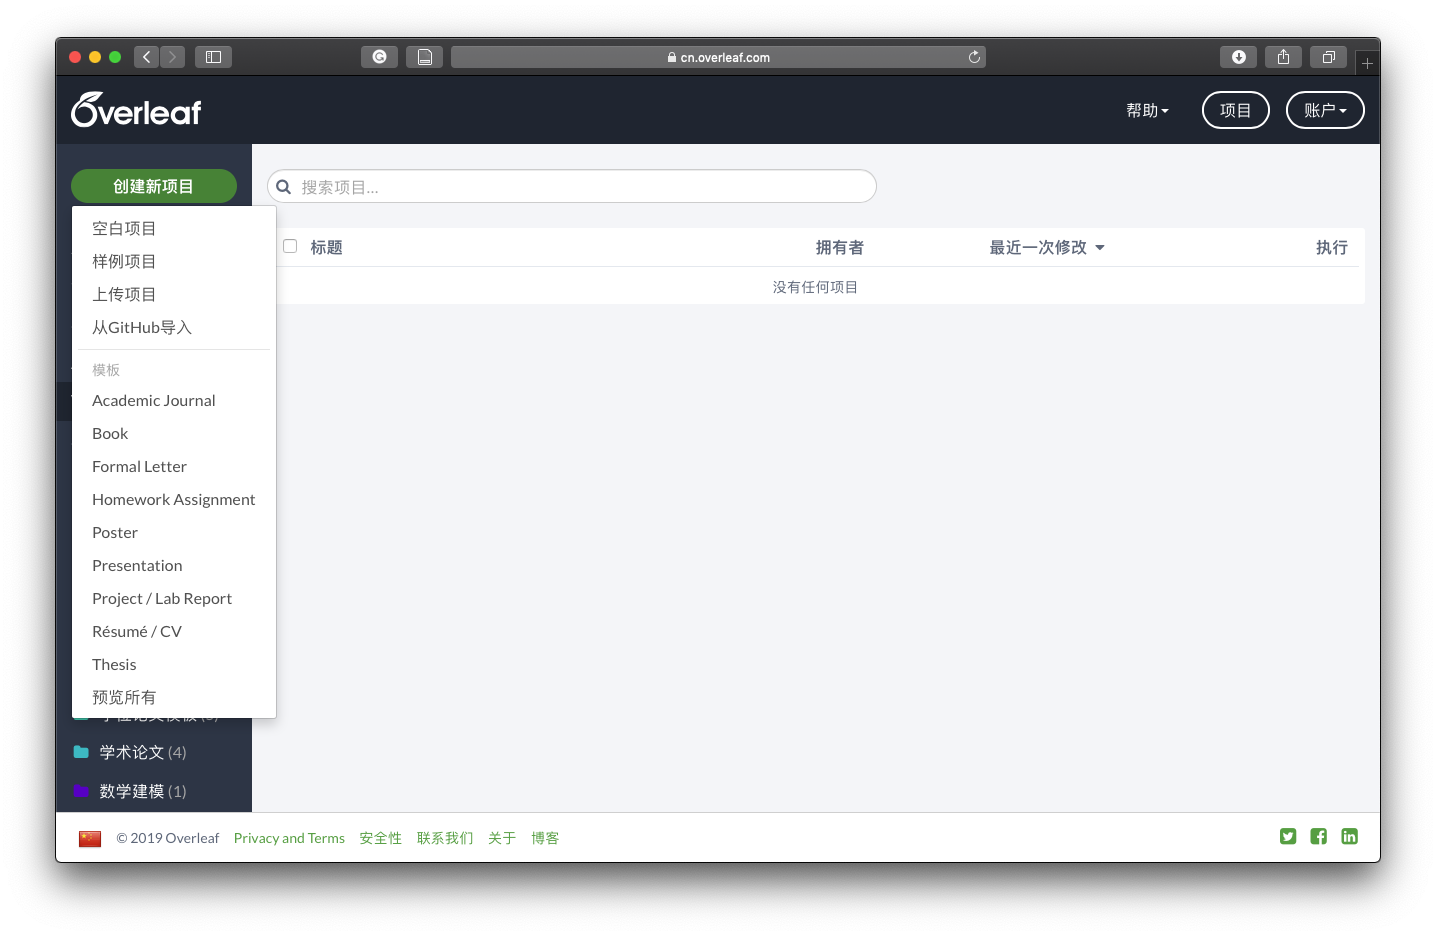
\includegraphics{figure/newproject.png}
\caption{新建项目}
\end{figure}

空白项目:一个空的项目,没有内容.

示例项目:一个简单示例项目,包含图片、参考文献的插入.

上传项目:我们之前可能有正在写作,还没有完成的项目.只要把所有文件压缩到一个.zip文件,上传即可.

从GitHub导入:

第\ref{template}章整理了一些发布在GitHub上的tex模板,我们可以直接fork到自己的账户下,然后在Overleaf中选择从GitHub导入.

(需要订阅才能关联GitHub账户)

(不订阅关联账户的话,只需要从GitHub下载.zip再通过上传项目即可)

除此之外,Overleaf提供了丰富的模板资源,可以在这里查看:
\url{https://cn.overleaf.com/latex/templates}

\hypertarget{section-4}{%
\section{个人写作}\label{section-4}}

项目建好后,界面和其他的tex客户端几乎没有区别.
左侧是tex的源文件,右侧是生成的pdf文件.

\begin{figure}
\centering
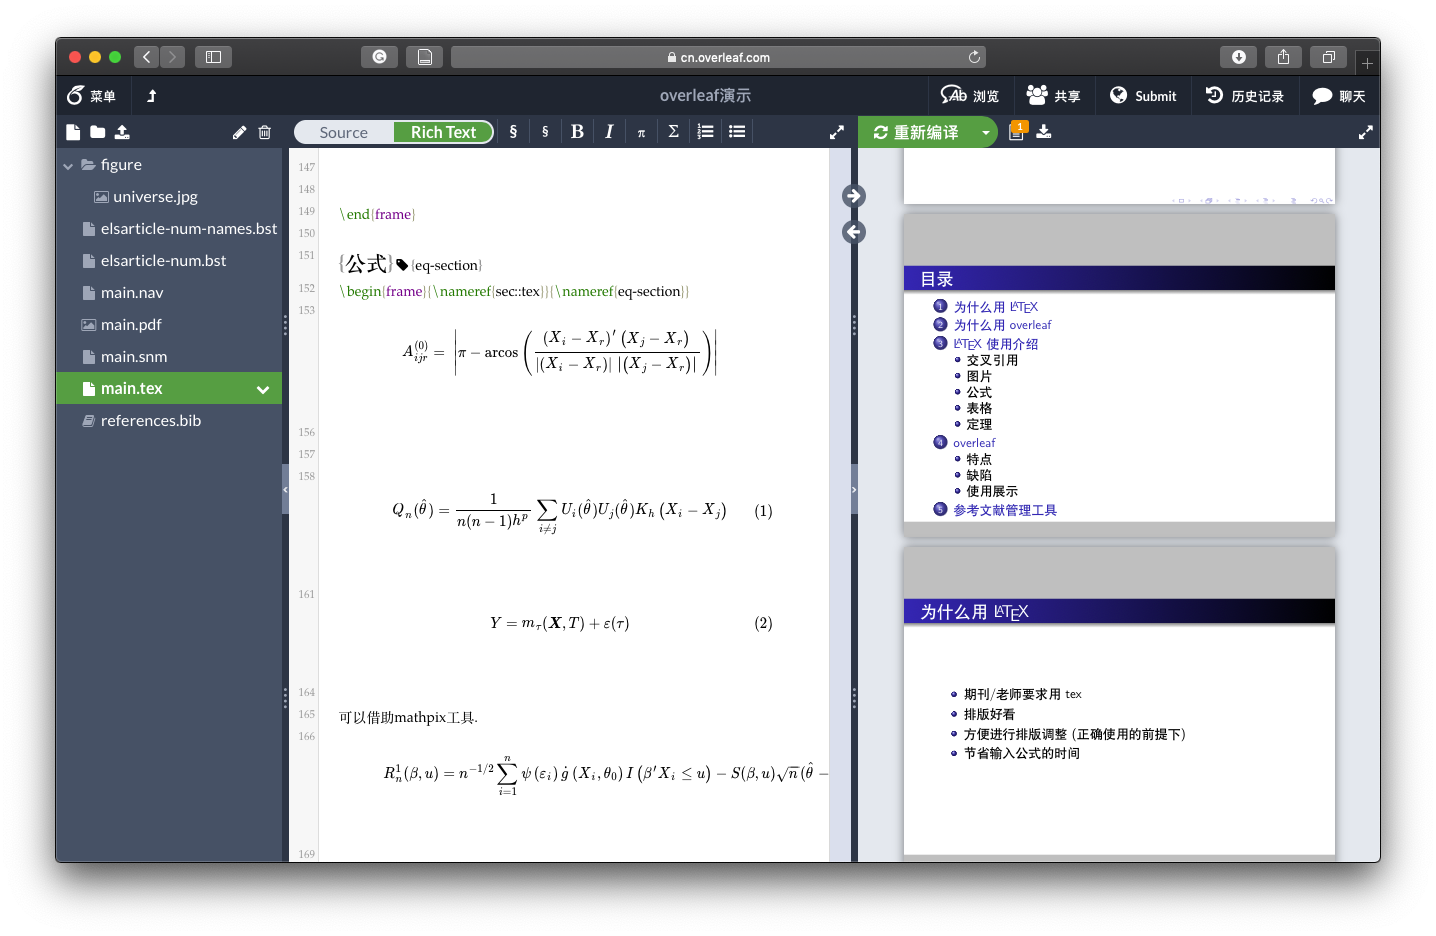
\includegraphics{figure/editepage.png}
\caption{编辑界面}
\end{figure}

详细的功能介绍在第\ref{basic}章介绍.

\hypertarget{section-5}{%
\section{添加参考文献}\label{section-5}}

关于参考文献的添加请看\ref{refe}节.

\hypertarget{section-6}{%
\section{邀请合作者}\label{section-6}}

右上角可以看到一个 \textbf{共享} 的功能,点击可以通过链接分享项或者通过账号邀请(免费用户只有1个合作者限制).
接下来就可以一起编写文章.

详细的说明在\ref{collaborator}.

\begin{figure}
\centering
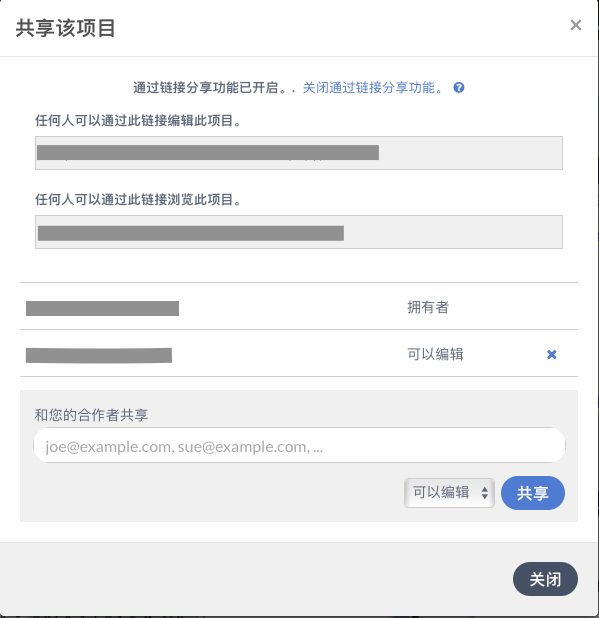
\includegraphics{figure/share.png}
\caption{share}
\end{figure}

链接分享就是只要通过链接,任何人都可以查看或修改项目.比如在第\ref{Overleafproject}章,我通过链接分享了一个beamer的示例项目.

\hypertarget{section-7}{%
\section{聊天}\label{section-7}}

右上角有个 \textbf{聊天} 功能,主要用于合作者之间交流.这个功能对于我们可能用途不是很大,需要交流的话我们可以选择微信、QQ等其他方式.

\hypertarget{section-8}{%
\section{论文投递}\label{section-8}}

论文写完后,右上角有 submit 功能,可以直接提交到期刊(现在已接入的较少).

当然,也可以下载源文件和pdf,具体请看\ref{downloadsource}节.

\begin{figure}
\centering

\includegraphics{figure/submit.jpg}
\caption{submit}
\end{figure}

\hypertarget{basic}{%
\chapter{基本功能}\label{basic}}

创建项目之后,我们进入到项目的编辑界面,如下图所示:
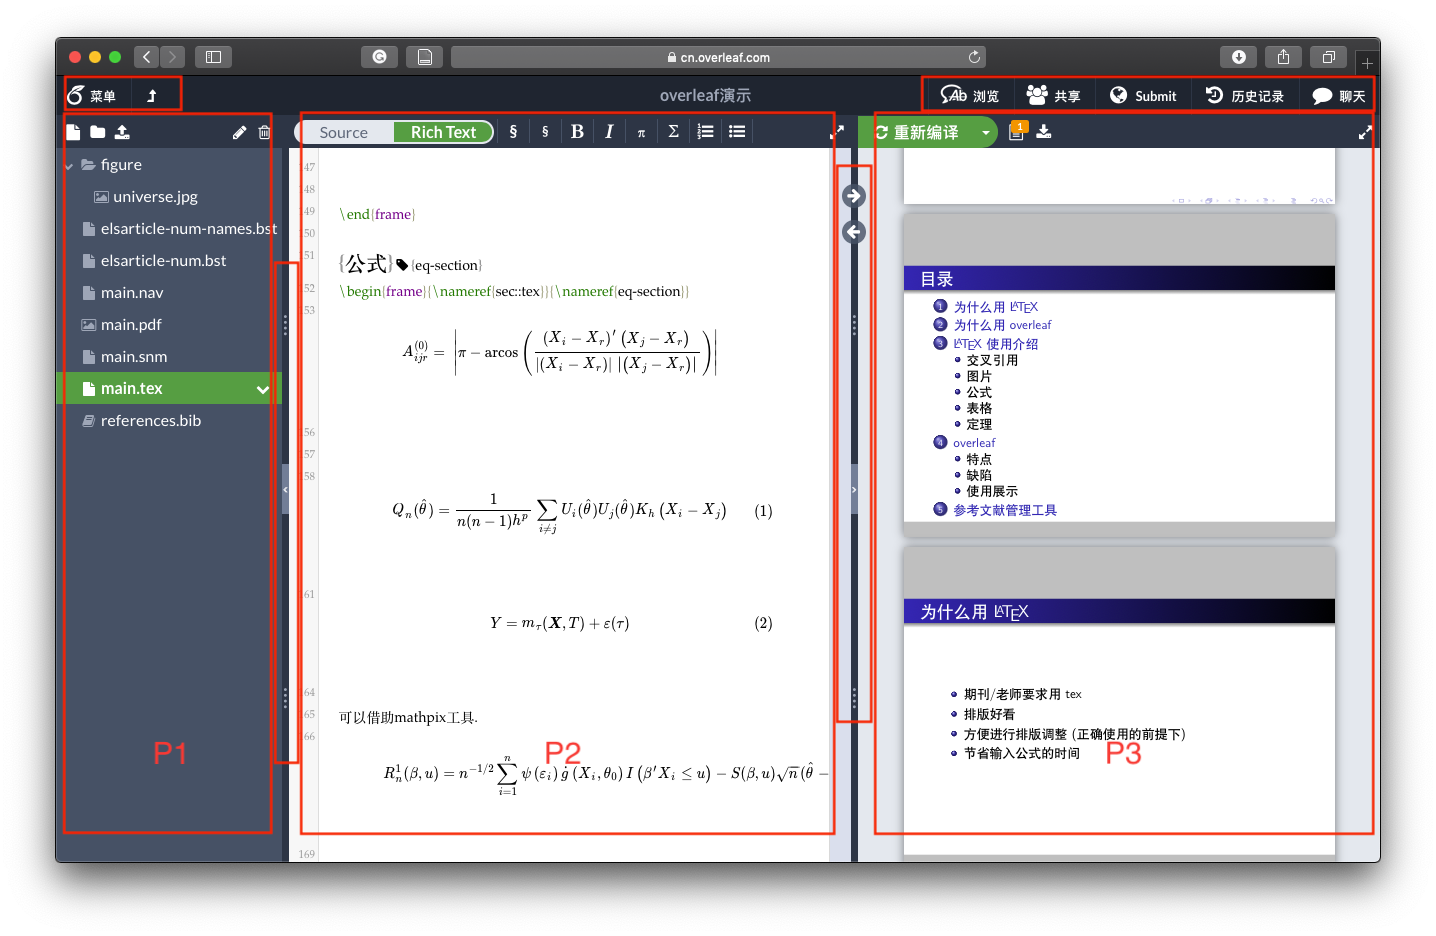
\includegraphics{figure/editepagemarked.png}

大块的划分主要可以分成4部分,分别是左侧的 \textbf{文件目录(P1)}、中间的\textbf{tex源文件(P2)}、右侧的\textbf{pdf预览(P3)}以及最上面有一条\textbf{菜单栏}.

P1、P2之间的分界线上有一些图标,其中 拖动\textbf{三个点}可以调整不同区域的大小, 点击中间的 \textbf{向左的箭头}可以隐藏文件目录P1.
类似的,在P2、P3之间也有相应的图标,可以设置隐藏pdf.另外P2、P3之间上方还有两个双向的箭头.他们的功能是在源文件和pdf之间跳转.比如我想看正在编写的这一页对应的pdf什么效果,点击向右的箭头就可以跳转到左侧光标所在位置对应的pdf页面.向左的箭头类似,可以跳转到正在查看的pdf所对应的tex源文件的位置,方便修改时定位.

\hypertarget{section-9}{%
\section{菜单栏}\label{section-9}}

菜单栏被项目名称从中间隔开,分成左右两部分.

其中右边 \textbf{共享}、\textbf{Submit}和\textbf{聊天}在第\ref{intro}章已经介绍过,剩下的\textbf{浏览}和\textbf{历史版本}在\ref{filehistory}节介绍.

关于左侧的菜单,\textbf{向上的箭头}用于退出当前项目,返回所有项目的列表.
点开\textbf{菜单}键,可以看到下面的结果:
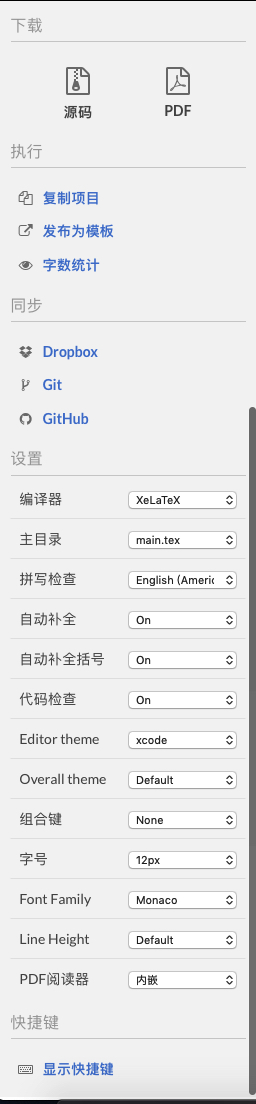
\includegraphics{figure/menu.jpg}

\hypertarget{downloadsource}{%
\subsection{下载}\label{downloadsource}}

如果需要下载tex源文件的话,只能从点开\textbf{菜单}下载.如果只是下载pdf的话,也可以点击右侧\textbf{P3}区域的下载图标.

\hypertarget{section-10}{%
\subsection{执行}\label{section-10}}

这里比较有用的可能只有 \textbf{字数统计} 功能,如下图:

\includegraphics{figure/wordcount.png}

\textbf{发布为模板}就是把当前的项目上传到Overleaf的模板库中.

\textbf{复制项目}就是复制一个相同的项目,比如我们通过链接打开别人分享的Overleaf模板,需要复制到自己的账户下使用.

\hypertarget{section-11}{%
\subsection{同步}\label{section-11}}

这里的功能需要订阅才能关联其他应用账号,主要在\ref{sync}节介绍.

\hypertarget{set}{%
\subsection{设置}\label{set}}

这里包括两部分设置,一部分是关于界面的个性化设置,比如字体、字号、界面主题等.另一部分是关于tex项目的设置,比如编译器,主目录等.

关于编译器的设置,简单讲,中文的文档设置XeLaTeX,英文文档设置pdfLaTeX.

(pdfLaTeX的编译效率会高一点,但是不支持中文.)

主目录在项目中有多个tex文件时需要设置,指定哪个文件是main.

\hypertarget{section-12}{%
\subsection{快捷键}\label{section-12}}

最下面有快捷键的说明,和常用的编辑器快捷键设置基本相同.
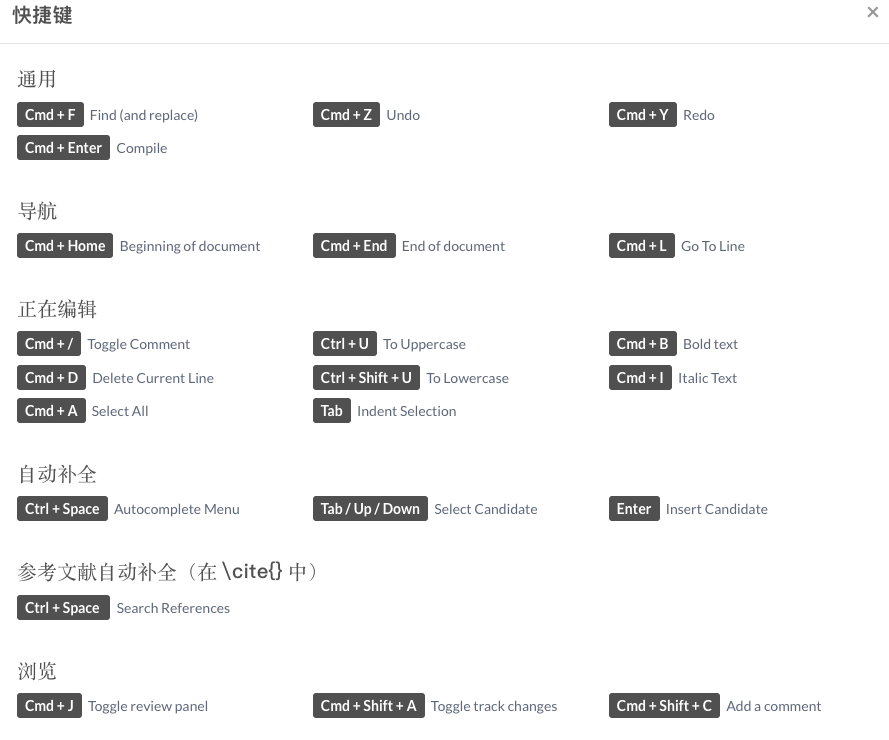
\includegraphics{figure/hotkey.png}

\hypertarget{p1}{%
\section{文件目录(P1)区域}\label{p1}}

\begin{figure}
\centering
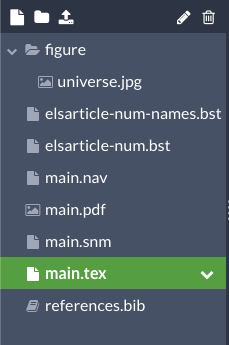
\includegraphics{figure/P1.png}
\caption{文件目录}
\end{figure}

当我们的文章需要插入很多图片、程序代码时,全在主目录下展开会显得比较乱.可以创建文件夹,用于存放文章中需要插入的材料.这就是这一区域的主要功能.

这一区域最上面有5个图标,下面是当前项目的文件目录结构.

5个图标从左开始,分别为:\textbf{新建文件,新建目录,上传,重命名,删除}.用于管理项目的文件结构.

\begin{figure}
\centering
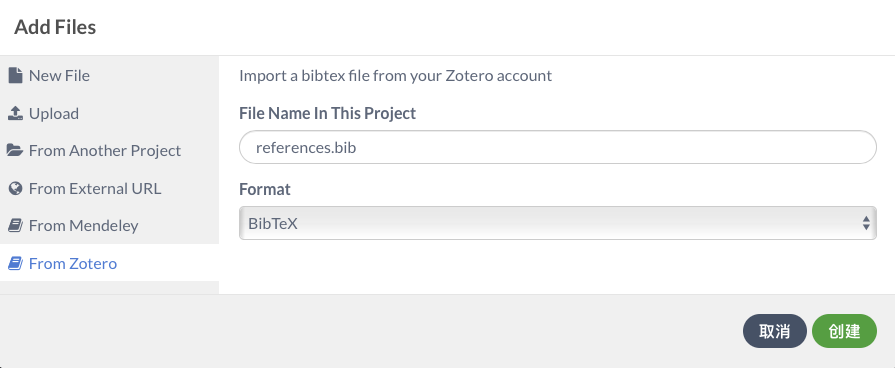
\includegraphics{figure/addfiles.png}
\caption{添加文件}
\end{figure}

(新建文件和上传点开都是这个界面 = =)

支持新建文件,上传文件,从链接下载以及从关联的账号直接导入.
在\ref{refe}节会演示关联zotero后添加参考文献bib文件.

\hypertarget{texp2}{%
\section{tex源文件(P2)区域}\label{texp2}}

\begin{figure}
\centering
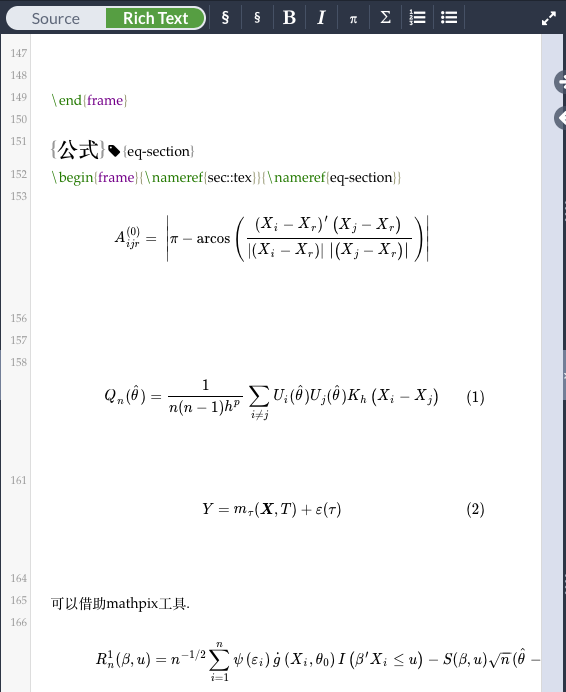
\includegraphics{figure/P2.png}
\caption{添加文件}
\end{figure}

这个区域主要用于输入内容,和tex客户端的主要区别是:
1.除了source之外,有一个Rich Text;
2.缺少了很多快捷插入的环境(目前只支持新建section、subsection,粗体,斜体,行内公式,行间公式,有序号枚举,无序号枚举).

另外,当我们开启右上角的 \textbf{浏览} 功能,这个区域会有所变化,在\ref{filehistory}节介绍.

source和常用的客户端中的展示效果一样,只是纯文本的源文件.

Rich Text可以得到类似Word那种效果,可以在源文件中看到编译好的公式结果.像上面图中展示的.

\hypertarget{pdfp3}{%
\section{pdf预览(P3)区域}\label{pdfp3}}

\begin{figure}
\centering
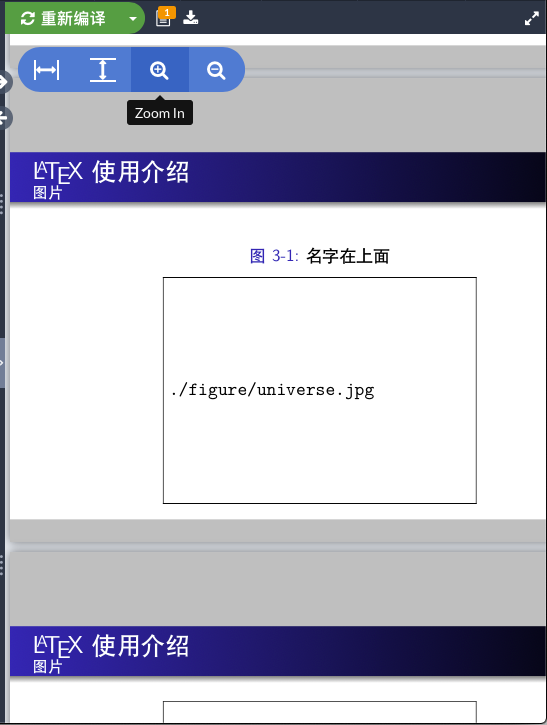
\includegraphics{figure/P3.png}
\caption{内嵌pdf预览}
\end{figure}

这一区域主要显示编译生成的pdf文件.最上面的3个菜单依次是 \textbf{编译模式设置}、\textbf{编译日志}、\textbf{下载pdf}.

如果只想下载pdf文件,不需要下载tex源文件,可以点击这一区域的下载图标.

如果在\ref{set}的设置中,pdf阅读器使用的是浏览器内嵌的,想要调整视图大小,可以将鼠标移动到pdf页面的左上区域,像上面图中的样子.如果设置的是本机,在苹果系统下,需要将鼠标移动到中间偏下的位置设置视图大小,如下图:

\begin{figure}
\centering
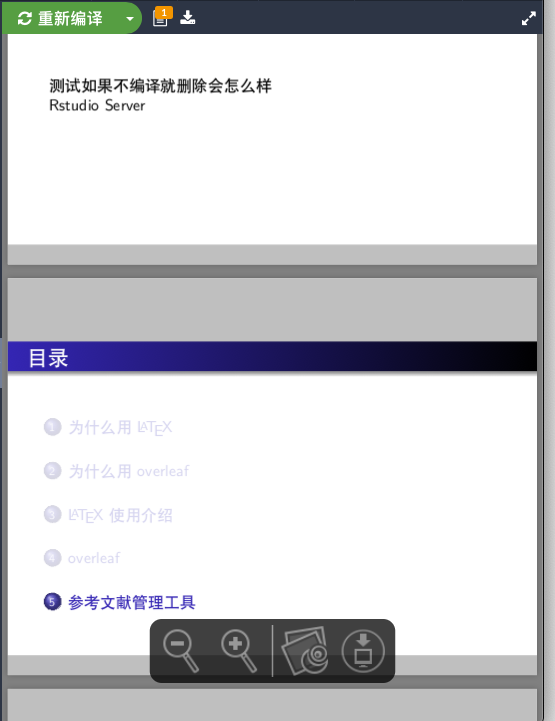
\includegraphics{figure/localpdf.png}
\caption{本机pdf预览}
\end{figure}

编译模式的设置如下图:

\begin{figure}
\centering
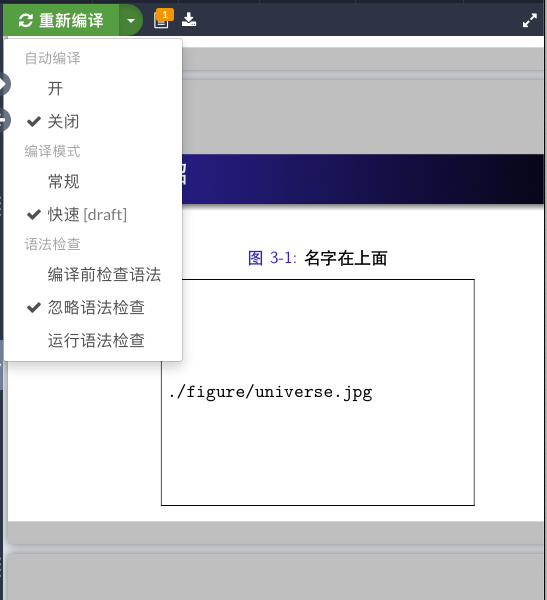
\includegraphics{figure/compileset.png}
\caption{编译设置}
\end{figure}

\textbf{自动编译}:就是只要左侧的源文件有变动,会自动编译(流量党请慎重打开).

\textbf{编译模式}:快速{[}draft{]}模式会省略一些效果,只显示主要内容,加快编译的速度.比如图中beamer的超链接和图片都没有正常显示.平时修改内容的时候可以选择draft模式,减少编译等待的时间,最后需要生成文件的时候,记得修改到常规模式.

\textbf{语法检查}:如果比较熟悉LaTeX的语法,也可以关掉,提高编译的速度.

\hypertarget{section-13}{%
\chapter{特色功能展示}\label{section-13}}

前面介绍的都是tex客户端所具有的基本功能,这章介绍一下Overleaf的特别之处.

需要订阅的会提示说明.

\hypertarget{sync}{%
\section{文件同步}\label{sync}}

不说多人合作的情况,就自己一个人的话,可能也会有多台设备.在多台设备之间同步文章撰写进度,需要网盘或者随身带u盘.

Overleaf利用网页技术,可以很方便的实现不同账户、不同设备之间的文件进度同步.

\hypertarget{section-14}{%
\subsection{个人本地和服务器同步}\label{section-14}}

\textbf{需要订阅}

订阅后可以关联Dropbox账号和GitHub账号,实现本地文件和服务器上的文件同步.

如果合作项目中,有多人正在同时编辑内容,本地修改会和网页修改发生冲突.

Dropbox服务不能直接使用.

关联GitHub账号主要方便导入和发布模板,其他用途不大.

\hypertarget{section-15}{%
\subsection{合作者之间同步}\label{section-15}}

合作者都通过网页版访问的话,每个人修改的内容会实时更新到文件中.

\hypertarget{collaborator}{%
\section{合作编辑}\label{collaborator}}

\textbf{不同套餐合作者数量限制不一样}

收到别人的项目邀请后,进入项目列表界面: \url{https://cn.overleaf.com/project}

会看到横幅通知:
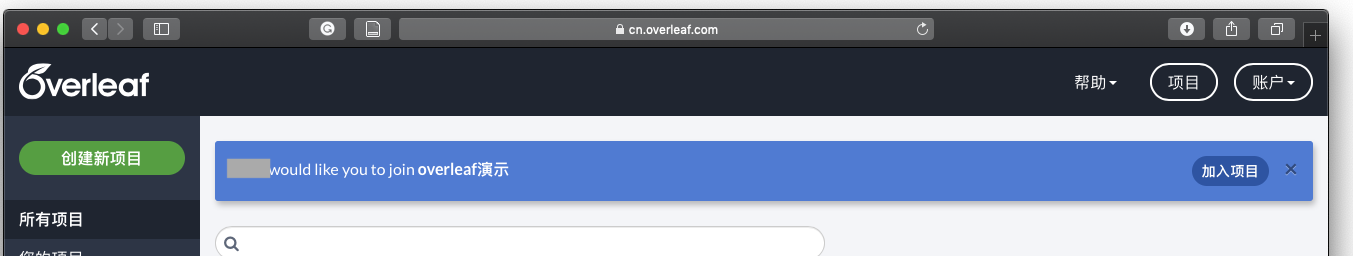
\includegraphics{figure/invite.png}
点击加入即可.之后这个项目会被归类到左侧 \textbf{与您共享的} 分类下.

在网页端,最上面可以看到正在这个项目中的人,像下面图中这样:

\includegraphics{figure/collaborator.png}

这时每个人的修改会被实时添加到项目中.

\hypertarget{filehistory}{%
\section{历史版本和修改记录}\label{filehistory}}

我们在写论文时,需要进行备份.比如最后论文完成时,可能会产生很多中间文件:XX第一版、XX第一版修改后\ldots{}

这些Overleaf都可以帮我们保存,而且还可以实现类似Word修订模式的修改记录.

\textbf{免费账户只能查看24h内的记录}

订阅后,可以保留项目的所有历史版本,可以对比不同版本的差别(包括文件目录以及tex源文件).对于重要的版本,可以添加标签,方便后续查看.
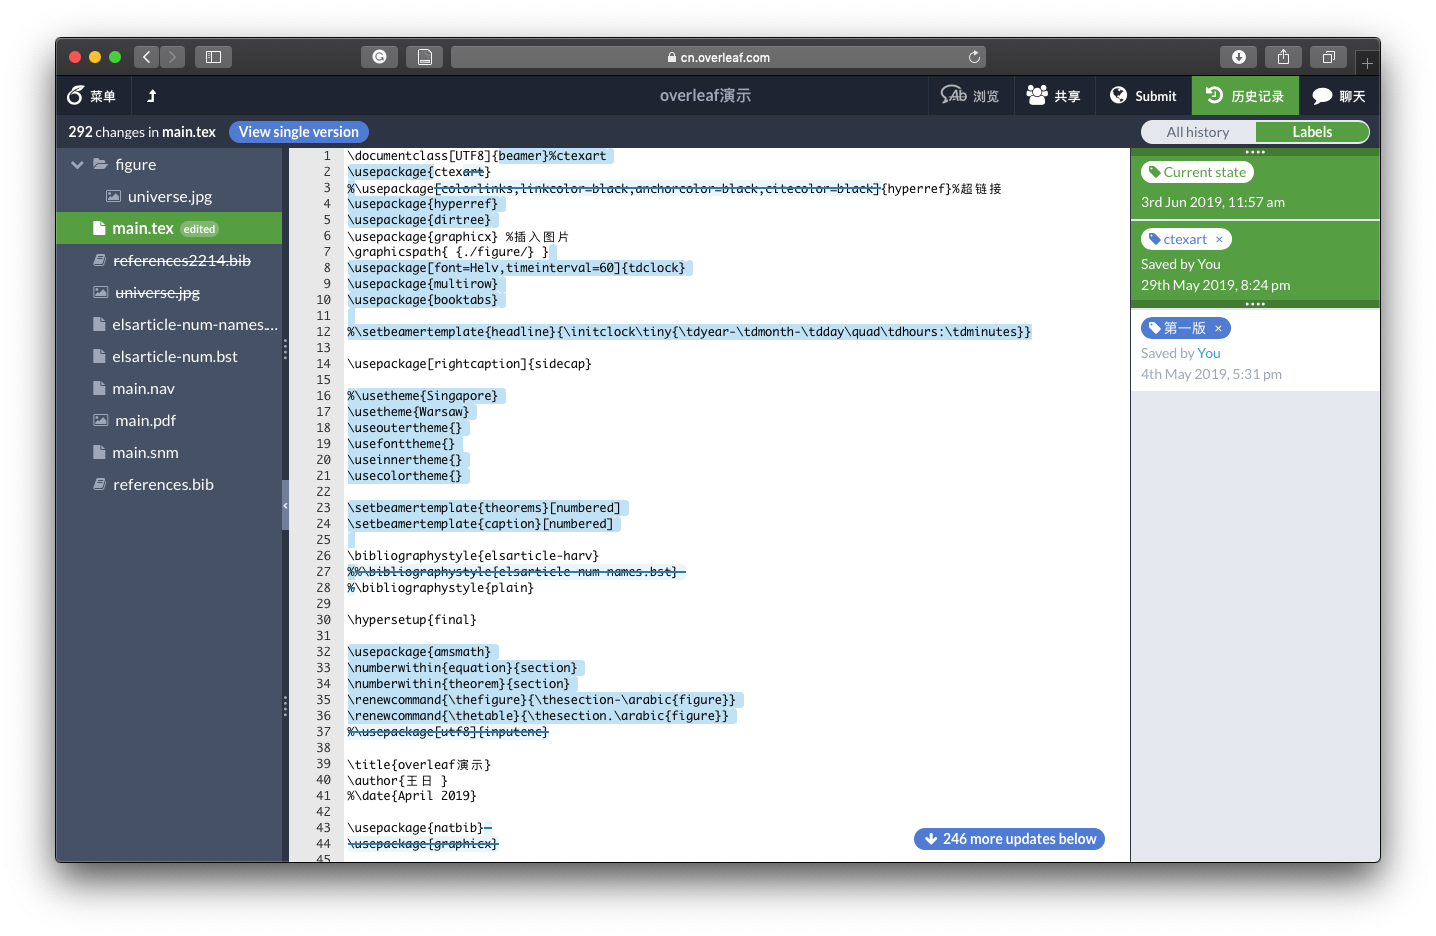
\includegraphics{figure/history.png}

\textbf{修改记录需要订阅}

下面这个界面可能很熟悉,借助网页技术,可以让LaTeX实现类似于Word修订模式的功能.
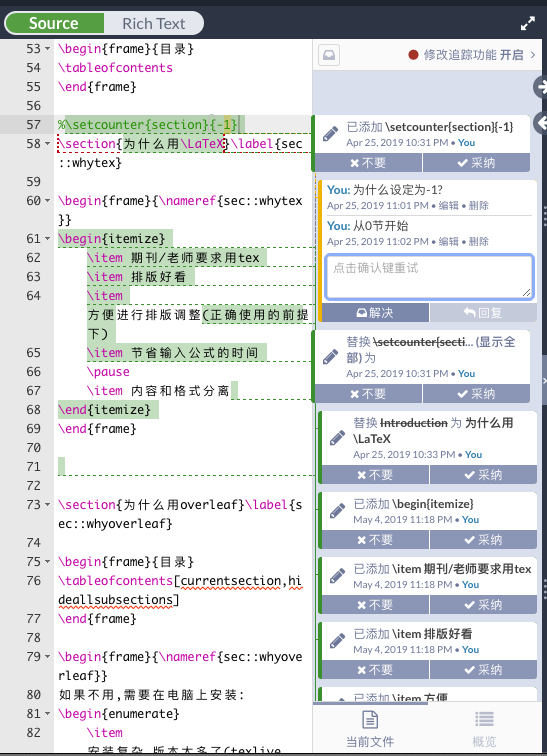
\includegraphics{figure/review.png}

\hypertarget{refe}{%
\section{参考文献整合}\label{refe}}

LaTeX写作,添加参考文献最便于修改的方案是BibTeX.

\url{https://liam.page/2016/01/23/using-bibtex-to-generate-reference/}
这里有详细的介绍.

简单讲这样的好处是:

1.参考文献中只会罗列正文中引用过的条目;

2.参考文献的引用形式以及排列方式有单独的文件控制.

\textbf{需要订阅才能关联zotero账户或者Mendeley账户}

当我们关联好参考文献的账户之后,选择 文件目录区域的添加文件

\begin{figure}
\centering
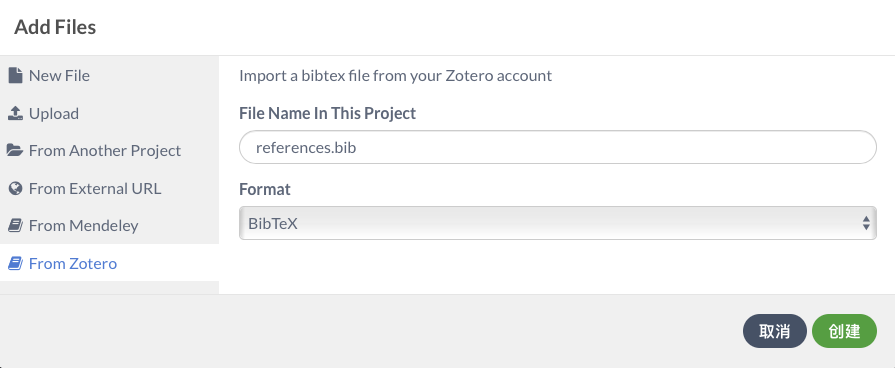
\includegraphics{figure/addfiles.png}
\caption{添加参考文献}
\end{figure}

文件名不一样不要在意,因为之前已经存在同名的文件了.

\begin{figure}
\centering
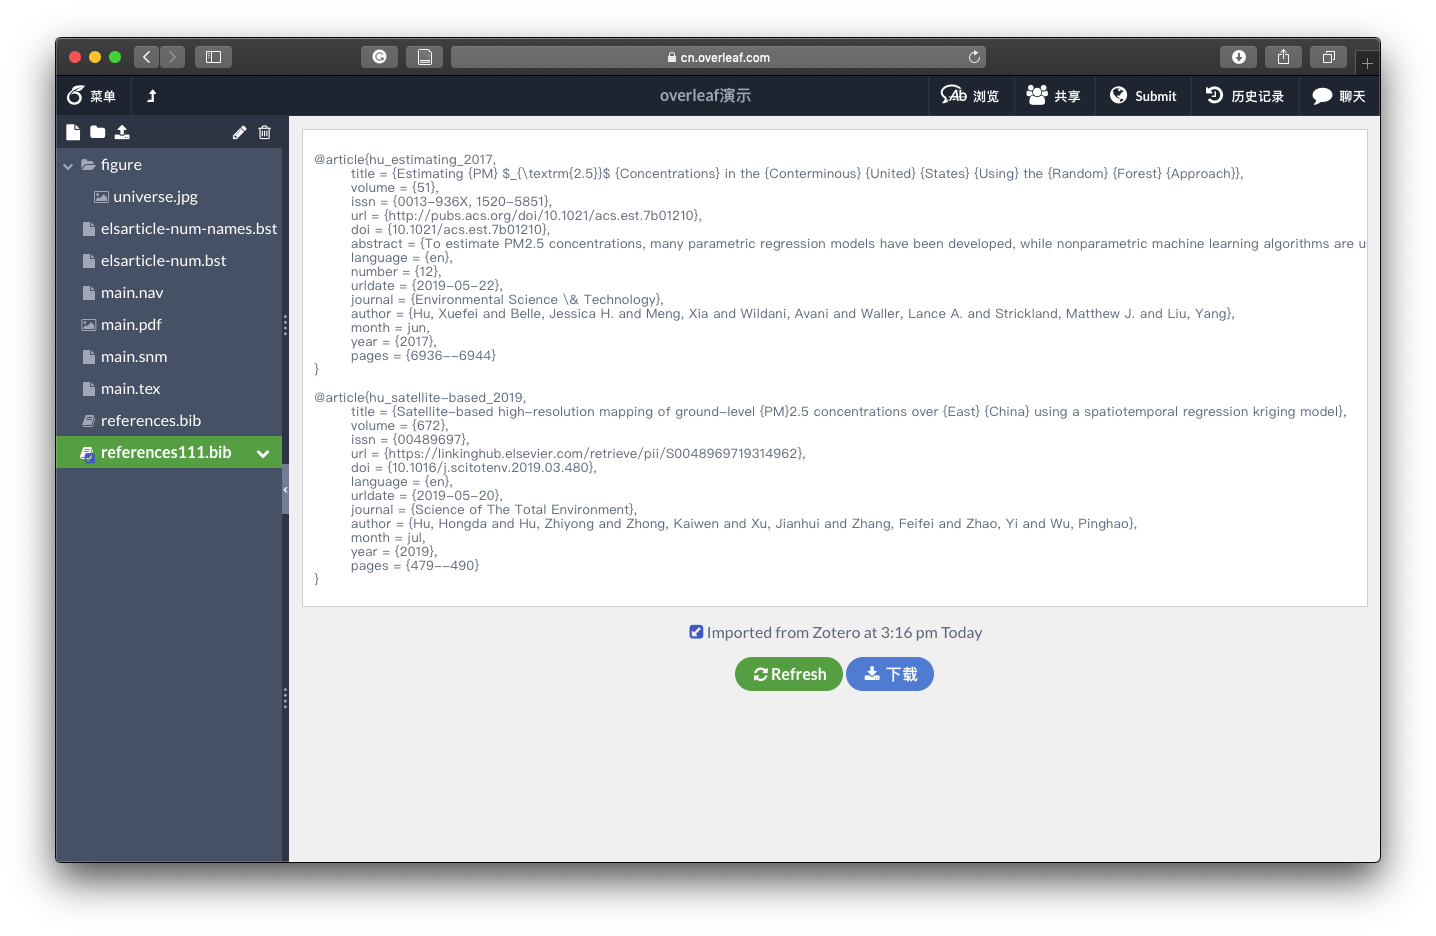
\includegraphics{figure/zotero.png}
\caption{zotero}
\end{figure}

这样当我们在zotero账户中添加新的文献后,只要打开这个文件点击Refresh即可.

(不订阅的话只不过需要手动导出bib文件再上传即可)

\hypertarget{section-16}{%
\chapter{缺陷}\label{section-16}}

\hypertarget{section-17}{%
\section{依赖网络}\label{section-17}}

这是Overleaf的优点,也同时是缺点.

比如现在在国内的访问速度就不是很理想,网速慢很影响使用体验.

\hypertarget{section-18}{%
\section{订阅费用}\label{section-18}}

目前提供的套餐中,没有比较适合学生写毕业论文的套餐.

\url{https://www.overleaf.com/user/subscription/plans}

当然免费账户基本可以满足大部分需求,只不过稍微麻烦一点.

\hypertarget{section-19}{%
\section{没有文章结构}\label{section-19}}

客户端常见的一个功能是可以显示文章的结构,目前Overleaf还不支持.

这一点在文章较长时,体验非常不好.

\hypertarget{section-20}{%
\section{没有常用符号表}\label{section-20}}

客户端常见的一个功能是可以通过点击图标插入不熟悉的符号,但是这点目前Overleaf还没有.不过他们提供了一个2页的常用指令,可以从这里下载:

\url{https://www.overleaf.com/for/community/resources}

\hypertarget{Overleafproject}{%
\chapter{示例项目}\label{Overleafproject}}

这里通过链接分享一些示例项目.

beamer的示例项目:
\url{https://cn.overleaf.com/read/tpzfjkmsfwkw}

每一页的标题通过引用section的label,修改section的标题,所有页面的标题会自动修改.

\hypertarget{section-21}{%
\chapter{其他工具}\label{section-21}}

这里介绍一些可以提高LaTeX写作效率的其他工具

\hypertarget{section-22}{%
\section{公式}\label{section-22}}

mathpix

可以很方便的将图片公式转成LaTex形式,手写公式不太乱的话也是可以识别的.

\url{https://mathpix.com}

\hypertarget{section-23}{%
\section{表格}\label{section-23}}

在LaTeX中插入表格并不是很简单的一件事,尤其是当表头需要合并单元格时.
这里介绍一些可以提高输入表格效率的工具.

\hypertarget{xtable}{%
\subsection{xtable包}\label{xtable}}

在R中进行模拟时,将结果输出至LaTeX可以利用这个包中的xtable函数.

\url{https://cran.r-project.org/web/packages/xtable/index.html}

\begin{Shaded}
\begin{Highlighting}[]
\NormalTok{xtable}\OperatorTok{::}\KeywordTok{xtable}\NormalTok{(}\KeywordTok{matrix}\NormalTok{(}\KeywordTok{rnorm}\NormalTok{(}\DecValTok{12}\NormalTok{),}\DecValTok{3}\NormalTok{,}\DecValTok{4}\NormalTok{))}
\end{Highlighting}
\end{Shaded}

\begin{verbatim}
## % latex table generated in R 3.6.0 by xtable 1.8-4 package
## % Tue Jun  4 15:28:46 2019
## \begin{table}[ht]
## \centering
## \begin{tabular}{rrrrr}
##   \hline
##  & 1 & 2 & 3 & 4 \\ 
##   \hline
## 1 & 0.48 & 0.75 & -0.18 & -0.66 \\ 
##   2 & 0.82 & -1.23 & 0.02 & -0.15 \\ 
##   3 & -0.09 & -0.49 & 0.95 & -0.46 \\ 
##    \hline
## \end{tabular}
## \end{table}
\end{verbatim}

这样我们直接粘贴到LaTeX中就可以了.

但是,这还不够.每次都要复制粘贴仍然很麻烦,而且如果表格的行名、列名有特定的格式,并不能直接粘贴结果(macOS下可以支持选择矩形区域修改).

我们可以利用LaTeX的\textbackslash{}input\{\}指令,完成更酷的操作.

大致流程就是在R中将xtable的输出结果写入文本文件``tableXXXX.tex'',然后在tex中需要插入表格的地方\textbackslash{}input\{tableXXXX.tex\}.

这样我们每次要把R新计算出来的表格更新到tex中,只需要重新编译一次即可.

关于复杂表头的设计,可以参考这个回答:

\url{https://stackoverflow.com/questions/15036754/r-package-xtable-how-to-create-a-latextable-with-multiple-rows-and-columns-from}

可以从:
\url{https://github.com/Ri0016/table-update-tex}
下载示例程序.

\hypertarget{excel2latex}{%
\subsection{Excel2LaTeX}\label{excel2latex}}

可以在Excel中合并好单元格,导出tex的表格.

\url{https://github.com/krlmlr/Excel2LaTeX/releases}

\hypertarget{latex}{%
\subsection{LaTeX中合并单元格}\label{latex}}

不知道tex合并单元格的命令可以在这个页面生成表格的tex代码:

\url{http://www.tablesgenerator.com/\#}

\hypertarget{template}{%
\chapter{一些模板}\label{template}}

\hypertarget{section-24}{%
\section{学位论文模板}\label{section-24}}

\url{https://github.com/ustctug/awesome-latex-thesis}

\hypertarget{elegantlatex}{%
\section{ElegantLaTeX}\label{elegantlatex}}

\url{https://github.com/ElegantLaTeX}

\hypertarget{beamer}{%
\section{beamer主题}\label{beamer}}

\url{http://deic.uab.es/~iblanes/beamer_gallery/index_by_theme.html}

\url{https://www.namsu.de/latex/themes/outer.html}

\cleardoublepage

\hypertarget{appendix-}{%
\appendix \addcontentsline{toc}{chapter}{\appendixname}}


\hypertarget{sound}{%
\chapter{余音绕梁}\label{sound}}

呐,到这里朕的书差不多写完了,但还有几句话要交待,所以开个附录,再啰嗦几句,各位客官稍安勿躁、扶稳坐好。

\bibliography{book.bib,packages.bib}

\backmatter
\printindex

\end{document}
